\renewcommand{\chaptername}{Chapter} 
\chapter{Limitations and Challenges in Estimating Internal Noise}\label{chap5}

In our study in chapter \ref{chap4}, analyzing the representation + noise data enabled us to distinguish distinct pathological profiles and uncover the diverse sensory and cognitive mechanisms underlying prosody processing impairments after stroke. Since not all patients exhibited deficits in both parameters, examining extreme cases provides insight into the potential neurological bases of these abnormalities. However, are these cases truly extreme, or are we simply unable to accurately estimate their impairments? It is possible that their excessive responses do not align with the average pathological profiles, leading to misclassification. 

\section {Perseveration as a challenge to Internal Noise Estimation} 

By examining responses closely, we observe that some patients consistently chose the same stimulus across multiple trials without variation. As previously discussed, this behavior may result from attentional challenges following right-hemisphere stroke or symptoms of spatial neglect. This pattern has also been notably observed during speech and language therapy (SLT) sessions by therapists, further highlighting its clinical relevance. 

From the perspective of the linear observer model and signal detection theory, participants exhibiting perseverative behavior no longer rely on their decision model to guide their responses. Instead of making choices based on their mental representation, they disengage from actively applying it to the stimuli. As a result, their responses become detached from stimulus evaluation, suggesting a lack of attentional control in determining which stimulus should be chosen.

Several established tasks exist for quantifying perseveration, such as Object Alternation (OA) \cite{freedman_orbitofrontal_1998} and the Wisconsin Card Sorting Test (WCST) \cite{abbruzzese_performance_1996}, which are widely used in assessing cognitive rigidity in conditions like aphasia and schizophrenia. These tasks measure executive function impairments, including difficulty in adapting to rule changes and excessive response repetition. However, despite their use in broader neuropsychological research, they have not been systematically applied to evaluate prosody perception deficits after stroke. Investigating whether similar mechanisms of perseveration extend to prosodic processing could provide new insights into the relationship between executive function deficits and speech impairments in stroke patients.


In the double-pass experiment, excessive responses may occur in repeated trials, potentially leading to false probabilities of agreement, making them appear to have low internal noise, despite poor cognitive flexibility. Conversely, if these behaviors do not manifest within the repeated trials, they may go undetected by internal noise estimates, leading to underestimation of internal noise. Additionally, because our kernel estimation relies on the average of responses, some patients may appear to have representations similar to controls, despite underlying perseverative tendencies. This raises the question of whether our regression-based method for classifcation images is truly optimal or if it leads to an over- or underestimation of their deficits.


\begin{tcolorbox}[title=Palin Toolbox: Perseverating observer simulation,
    colback=white!30!white, colframe=blue!80!white]
In PALIN we have the possibility to simulate a perseverating observer that is not responding based on their decision model and repeating the same response as before based on a numerical matrix, for example, a participant that perseverates 30\% of the time. 

\tcblower

\begin{minted}[fontsize=\tiny]{python}
# Create a simple experiment
exp = SimpleExperiment(n_trials=150,trial_type=Int2Trial,
    n_features=7,external_noise_std=100)
# Initialize PerseveratingObserver with a random kernel
obs = PerseveratingObserver.with_random_kernel(
    n_features=exp.n_features,
    internal_noise_std=4,
    criteria=0,
    transition_matrix=[[0.9, 0.1], [0.01, 0.99]])
# Get response
responses = obs.respond_to_experiment(exp)
responses_df = Analyser.to_df(exp, responses)
\end{minted}

\end{tcolorbox}
\begin{figure}[ht!]
    \centering
    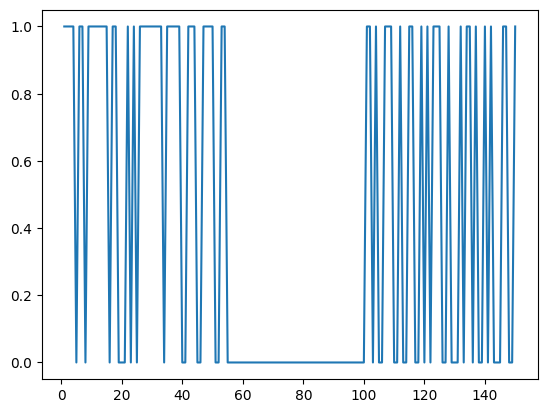
\includegraphics[width=10cm]{MainLayout/Images/perseveration.png}
    \caption{Main Title for First Image \\ \small Subtitle for the first graphic.}
    \label{fig:perseverating_observer}
\end{figure}


\section {Better internal noise}

Estimating internal noise using the double-pass paradigm, as described in Chapter \ref{chap3}, relies on a fundamental assumption: if the same stimulus is presented twice, an ideal deterministic observer (i.e., one with no internal noise) should respond identically in both passes. However, in real-world conditions, human observers exhibit response variability due to internal noise, leading to inconsistencies. To measure this variability, we analyze two key behavioral metrics:
\begin{itemize}
    \item Percentage of Agreement (Pa): The proportion of trials where the participant gives the same response in both passes.
    \item Probability of Choosing Interval 1 (Pint1): The proportion of trials where the participant selects response category 1 across all trials.
\end{itemize}

From these empirical values, internal noise and decision bias are estimated using Monte Carlo simulations. This method involves generating artificial observers that mimic human decision-making under different noise conditions. Each simulated observer follows the Signal Detection Theory (SDT) framework, where responses are influenced by:
\begin{itemize}
    \item A fixed decision criterion (bias) that determines the threshold for choosing one response over another.
    \item A level of internal noise that affects response variability.
\end{itemize}
In the simulation, a range of artificial observers is created, each with varying levels of internal noise and different response biases (favoring Interval 1 or 2). These simulated observers undergo a large number of trials, producing predicted values of (Pa, Pint1) for different noise and bias conditions. The next step involves comparing the participant’s actual (Pa, Pint1) values against the simulated dataset. The algorithm identifies the simulated observer whose (Pa, Pint1) values best align with the participant’s empirical data. This is achieved by minimizing the difference between the observed and simulated (Pa, Pint1) values. The internal noise (IN) and bias value that yield the closest match are selected as the final estimated parameters for the participant.

This method allows us to estimate perceptual variability and decision biases without relying on a traditional correct/incorrect response framework, as required in higher-level cognitive experiments like prosody perception tasks, where no objective ground truth exists. However, this approach also has limitations, particularly in stroke patients where perseveration, response biases, and fluctuations in attention can introduce additional noise sources that deviate from SDT assumptions, as discussed in prior sections.

Upper Limit Problem (>5):
Studies (e.g., Neri, 2010) suggest that noise estimates beyond IN > 5 should be considered unreliable.
If the estimated internal noise exceeds this range, the model may no longer capture perceptual variability but instead reflect response inconsistencies, such as perseveration, impulsivity, or lapses in attention.
A critical methodological limitation is that for participants exhibiting high internal noise, the estimated percentage of agreement (Pa) may approach chance levels, making it indistinguishable from completely random responses. In such cases, Monte Carlo simulations may fail to differentiate whether a patient genuinely exhibits pathologically high internal noise or if they are simply responding randomly due to task disengagement. The issue is exacerbated by the fact that, unlike low-level perceptual tasks where there is a correct or incorrect response, the present study involves a higher-level prosody classification task in which responses are subjective and based on an individual’s mental representation rather than an objective standard. This makes it even more challenging to attribute response variability solely to internal noise rather than to shifts in perceptual strategies.


Sampling Error \& Confidence Intervals:
With only 50-150 trials, the double-pass method may not provide sufficient resolution to accurately estimate internal noise above a certain threshold (e.g., IN = 5).
Monte Carlo simulations suggest that for values of IN > 5, increasing the number of trials (e.g., to 1000 or more) is necessary to get stable estimates.
In stroke patients, where trials are often limited due to fatigue or cognitive impairment, the estimation method might not capture their true perceptual variability.
When the number of double-pass trials is small (e.g., 50-150 trials), the variance in internal noise estimation increases.
Confidence intervals widen significantly, making it difficult to differentiate noise values above a certain threshold.
Empirical simulations show that IN estimates tend to be overestimated for values <6 and underestimated for values >6.
Another major methodological limitation arises from trial count restrictions. Estimating internal noise requires a substantial number of repeated trials for statistical reliability, yet in clinical populations such as stroke patients, lengthy experimental sessions are not feasible due to fatigue and attentional constraints. As a result, the limited number of trials introduces a high degree of variability in the estimated internal noise, making the measurement less reliable. Additionally, the method does not account for response perseveration, a phenomenon frequently observed in stroke patients with right-hemisphere damage. Perseveration can artificially inflate estimates of internal noise because the model assumes that repeated trials are independent, whereas in reality, some patients persistently select the same response across multiple trials regardless of the presented stimulus. This means that some patients may appear to have high internal noise simply due to habitual responding rather than perceptual instability.

Beyond these theoretical and methodological concerns, practical limitations also affect the applicability of Monte Carlo simulations in clinical settings. The estimation process requires large-scale simulations across a wide range of internal noise and bias values, making the approach computationally intensive. Running thousands of simulated trials to obtain stable estimates is feasible for offline analysis but becomes impractical for real-time clinical assessments where fast, efficient estimation methods are needed. Additionally, the method assumes that patient behavior conforms to the SDT framework, but in reality, some stroke survivors may demonstrate idiosyncratic decision-making strategies that fall outside of the model’s assumptions. This means that the estimated internal noise may not always reflect true perceptual variability but instead capture artifacts introduced by strategy shifts, attentional fluctuations, or cognitive rigidity.

Finally, the upper limit for internal noise estimation introduces additional concerns. When empirical values of (Pa, Pint1) approach the theoretical limit of infinite internal noise, the inference process breaks down. This can happen for two primary reasons: first, due to the limited number of repeated trials, which introduces sampling errors that artificially lower Pa, and second, due to the patient’s cognitive process diverging from the model assumptions, leading to behavioral patterns that the model cannot interpret correctly. As demonstrated in previous simulations, the number of trials required to reliably estimate high internal noise values increases exponentially, making the approach impractical for clinical applications. In cases where patients exhibit extremely low Pa values, the model struggles to differentiate whether this reflects true perceptual instability or merely a lack of task engagement, further reducing the reliability of the inferred estimates.


\section {Discussion} 
